\documentclass{article}
\newcommand\tab[1][1cm]{\hspace*{#1}}
\usepackage{gensymb}
\usepackage{graphicx}
\graphicspath{{./documents/}{./figs}}
\usepackage{multicol}
\begin{document}
\begin{enumerate}
	\item In the given figure, PQ is tangent to the circle centred at $\vec{O}$.If \angle{AOB}=$95^{\degree}$, then the measure of \angle{ABQ} will be
		\begin{figure}[h]
		\centering
	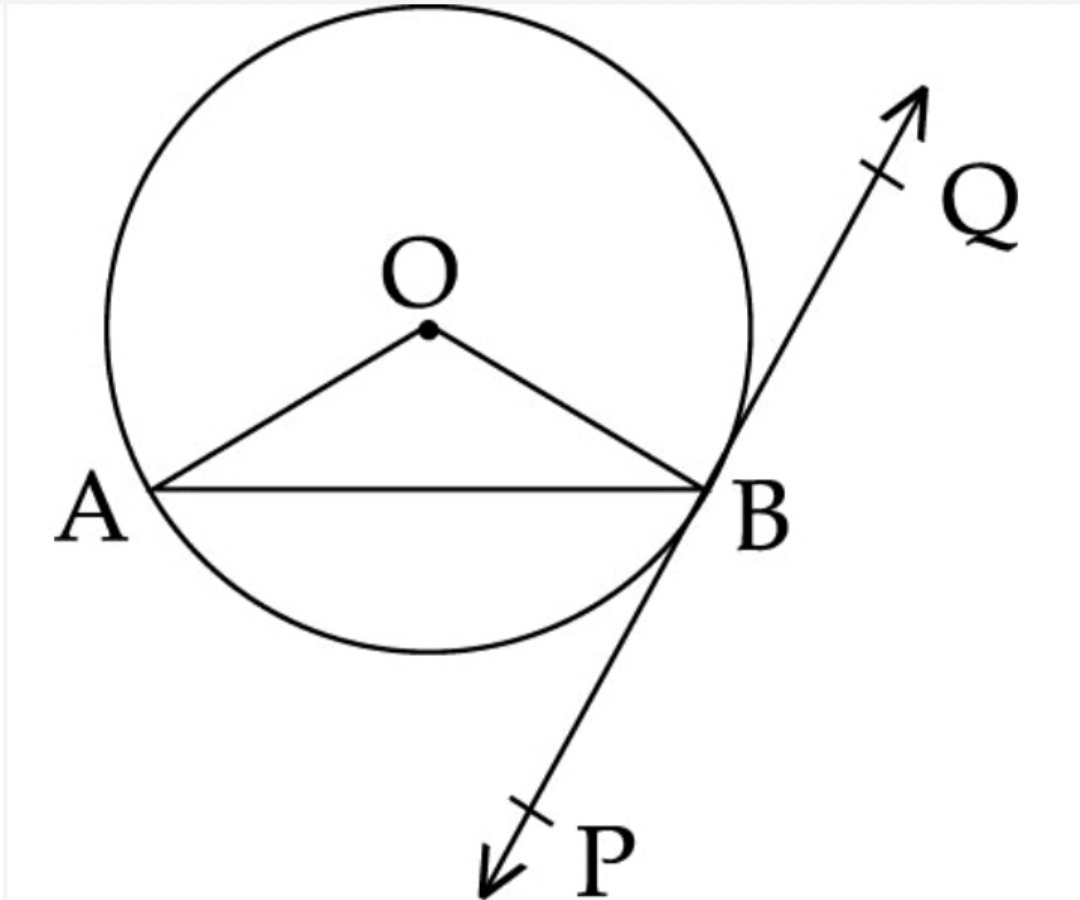
\includegraphics[width=0.3\columnwidth]{fig1.jpg}
		
\end{figure}
			\begin{enumerate}
				\item $47.5^{\degree}$
				\item $42.5^{\degree}$
				\item $85^{\degree}$
				\item $95^{\degree}$
		\end{enumerate}  

	\item (a) Two tangents TP and TQ are drawn to a circle with center $\vec{O}$ from an external point T. prove that \angle{PTQ}=2\angle{OPQ}
		\begin{figure}[h]
			\centering
			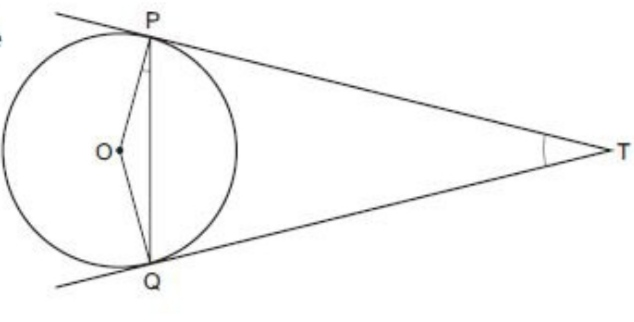
\includegraphics[width=0.35\columnwidth]{Fig2.jpg}
		\end{figure}
		$$\textbf{OR}$$
		(b) In the given figure, a circle is inscribed in a quadrilaterals ABCD in which \angle{B}=$90^{\degree}$. If AD=7 cm,AB=20 cm and DS=3 cm, then find the radius of the circle
		\begin{figure}[h]
			\centering
			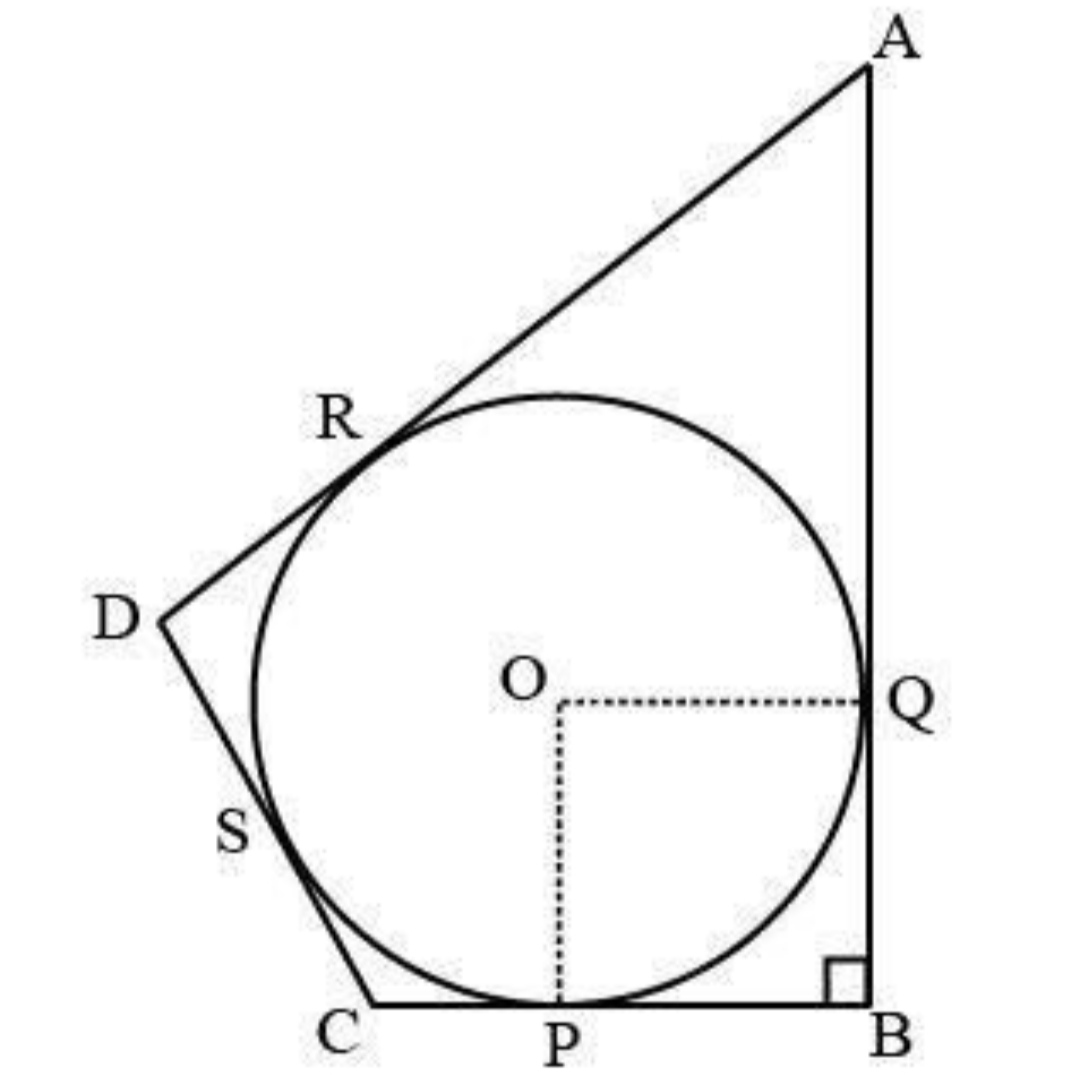
\includegraphics[width=0.35\columnwidth]{Fig3.jpg}
		\end{figure}
	\item The discus throw is an event in which an athlete attempts to throw a disus.the athlete spins anti-clockwise around one and a half times through a circle, then release the throw. when released,the discus travels along tangent to the circular spin orbit.
		\begin{figure}[h]
			\centering
			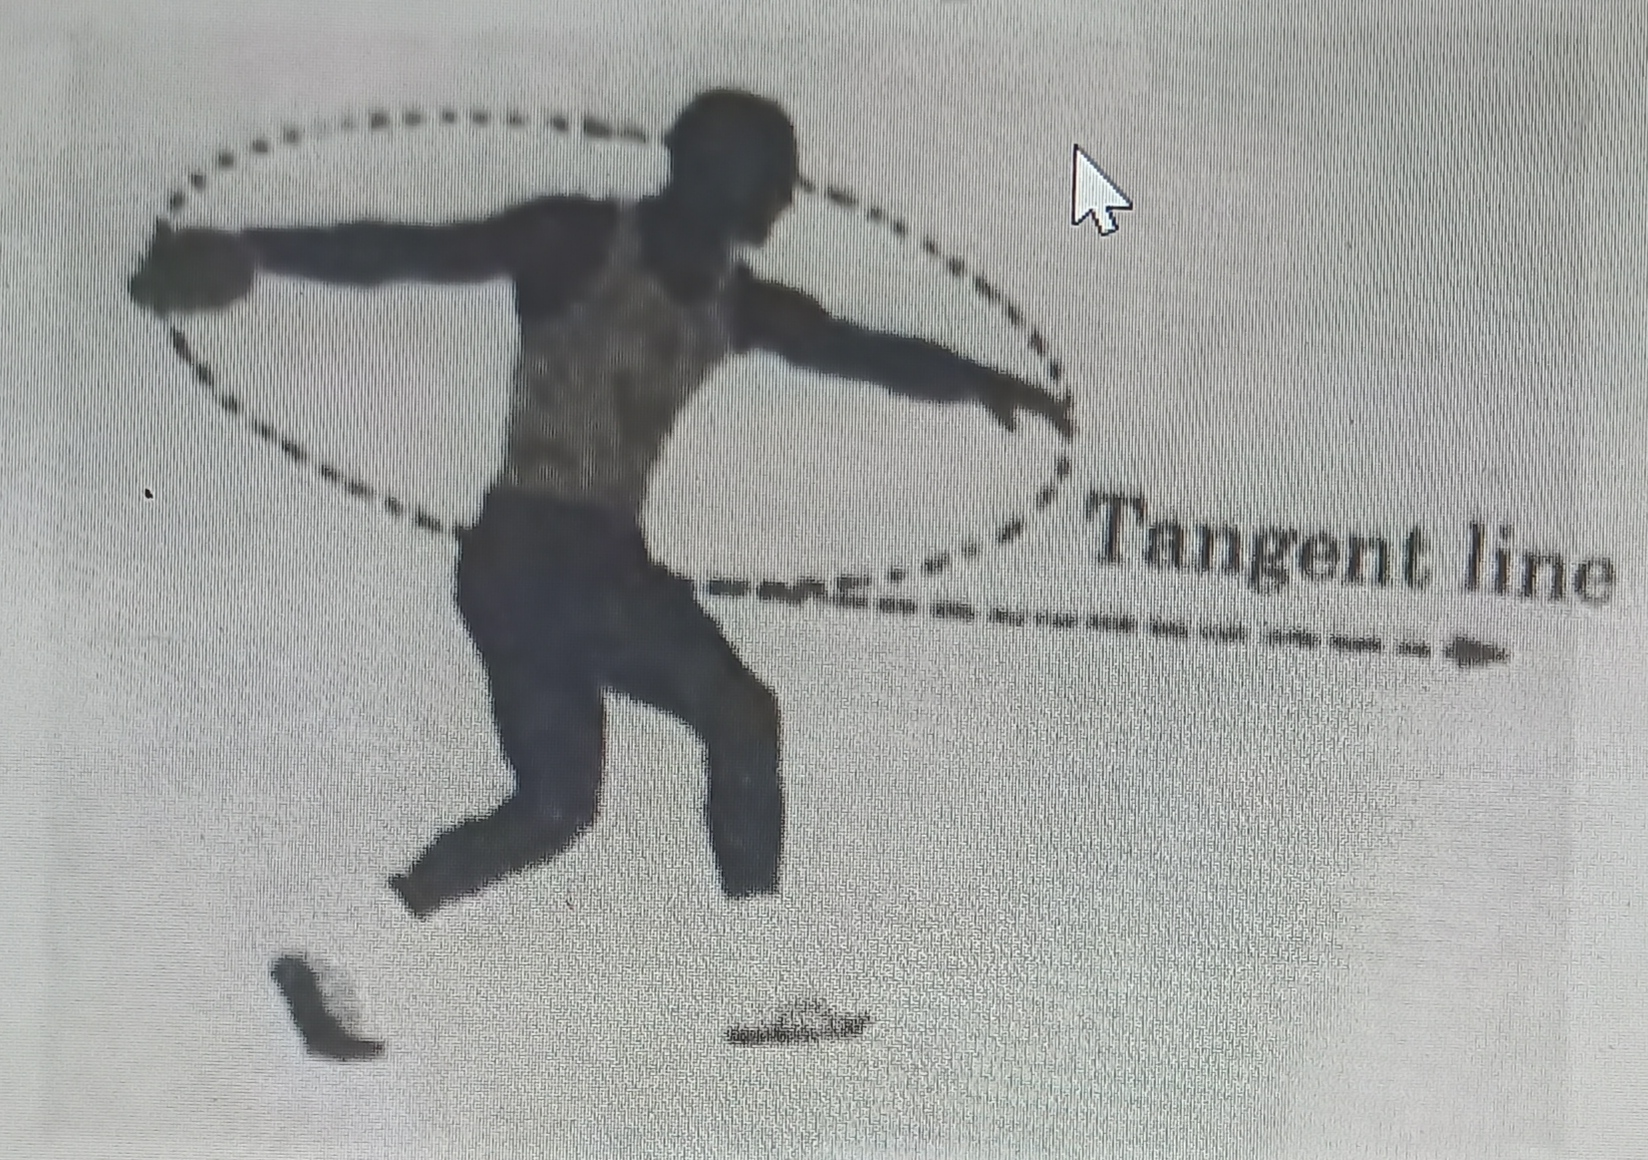
\includegraphics[width=0.35\columnwidth]{Fig4.jpg}
		\end{figure}\\
		In the given figure, AB is one such tangent to a circle of radius 75 cm.Point $\vec{O}$ is center of the circle and \angle{ABO}=$30^{\degree}$. PQ is parallel to OA
		\begin{figure}[h]
			\centering
			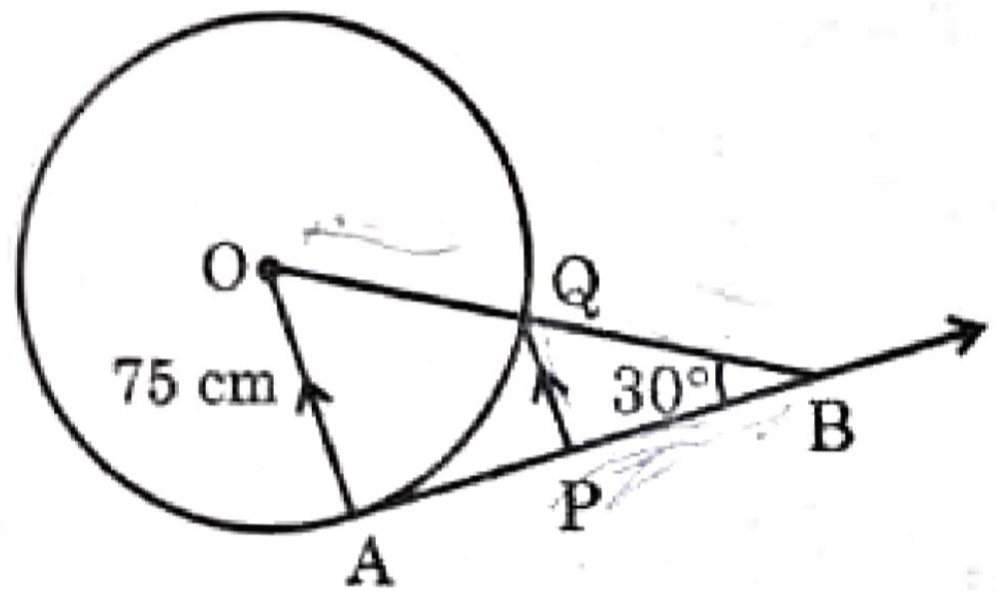
\includegraphics[width=0.35\columnwidth]{fig5.jpg}
		\end{figure}\\
		Based on above informtion:
		\begin{enumerate}
		\item find the length of AB.
		\item find the length of OB.
		\item find the length of PQ.
		\end{enumerate}
		\tab[2cm]OR\\
		\tab[0.75cm]find the length of PQ.
	\item In the given figure, the quadrilateral PQRS circumscribes a circle. Here PA+CS is equal to:
		\begin{figure}[h]
			\centering
			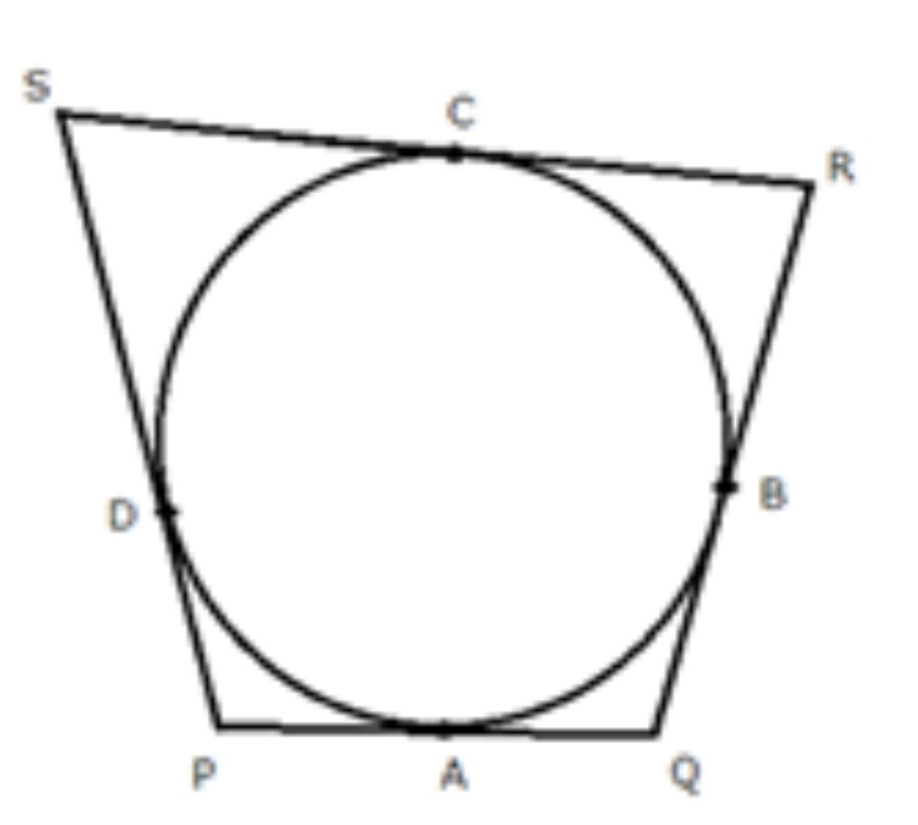
\includegraphics[width=0.35\columnwidth]{fig6.jpg}
		\end{figure}
		
			\begin{enumerate}
				\item QR
				\item PS
				\item PR
				\item PQ
			\end{enumerate}
		
		\item In the given figure, $\vec{O}$ is the center of the circle. AB and AC are tangents drawn to the circle from point A.If \angle{BAC}=$65^{\degree}$, then find the measure of \angle{BOC}.
		\begin{figure}[h]
			\centering
			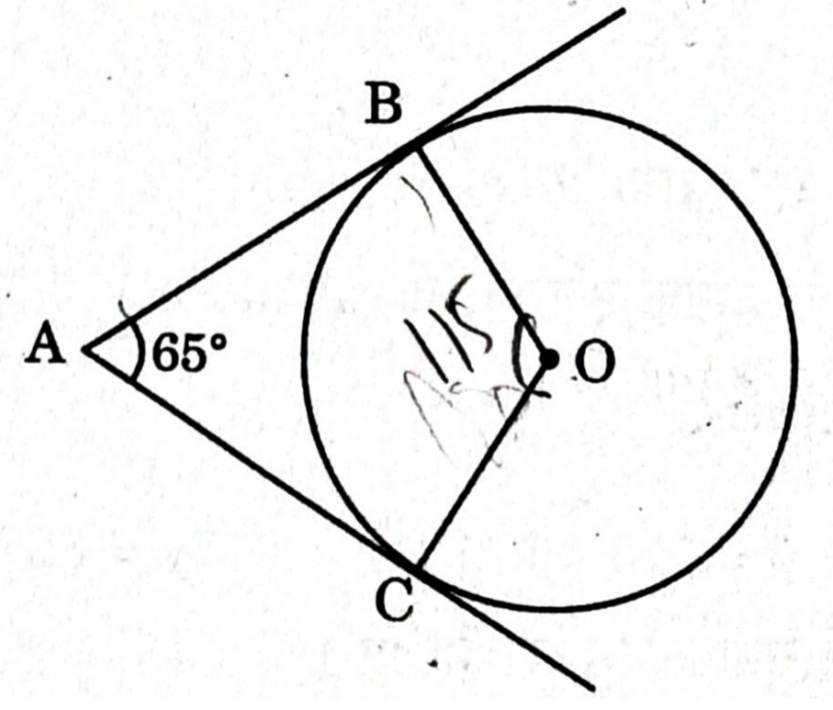
\includegraphics[width=0.35\columnwidth]{fig7.jpg}
		\end{figure}
	\item In the given figure, $\vec{O}$ is the center of the circle and QPR is a tangent to it at P. prove that \angle{QAP}+\angle{APR}=90$^{\degree}$
		\begin{figure}[h]
			\centering
			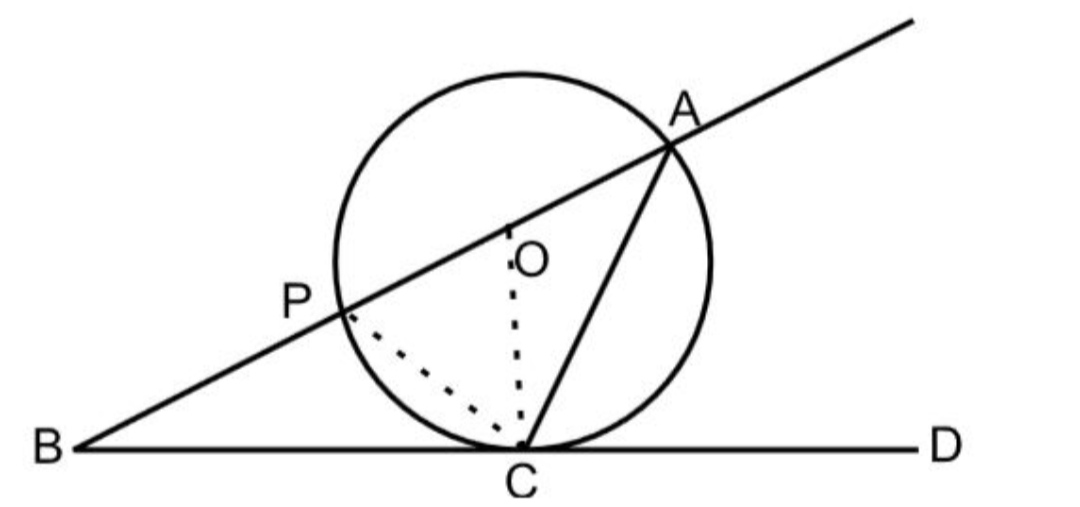
\includegraphics[width=0.35\columnwidth]{fig8.jpg}
		\end{figure}
	\item In the givien figure, PT is a tangent at T to the circle  with center $\vec{O}$.If \angle{TPO}=$25^{\degree}$, then x is equal to:
		\begin{figure}[h]
			\centering
			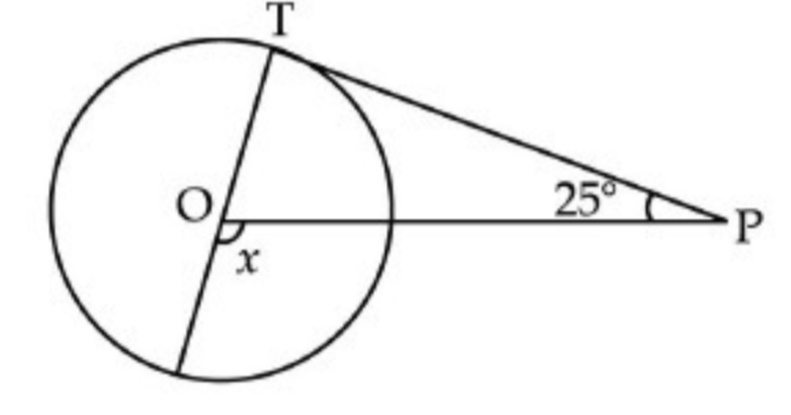
\includegraphics[width=0.4\columnwidth]{fig9.jpg}
		\end{figure}
		\begin{enumerate}
			\item $25^{\degree}$
			\item $65^{\degree}$
			\item $90^{\degree}$
			\item $115^{\degree}$
		\end{enumerate}
	\item In the given, TA is a tangent to the circle with center $\vec{O}$ such that OT=4cm, \angle{OTA}=$30^{\degree}$, then length of TA is:
		\begin{figure}[h]
			\centering
			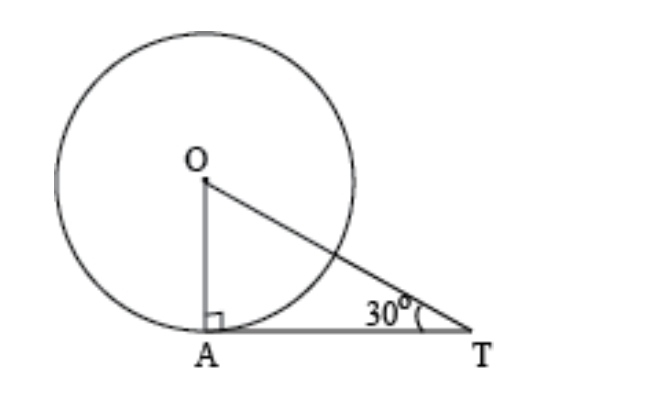
\includegraphics[width=0.6\columnwidth]{fig10.jpg}
		\end{figure}
	        \begin{enumerate}
			\item 2$\sqrt{3}$cm
			\item 2cm
			\item 2$\sqrt{2}$cm
			\item $\sqrt{3}$cm
		\end{enumerate}
	\item Two concentric circles are of radii 5cm and 3cm. Find the length of the chord of the larger circle which touches the smaller circle



\end{enumerate}
\end{document}
